\chapter{Methodology}
\label{cp:methodology}
\section{Apparatus} \label{sec:apparatus}

A system is set up to analyze the flow over an airfoil in a wind tunnel. This system begins with putting an airfoil in the test section, as seen in \autoref{fig:airfoil_in_tunnel}. \autoref{fig:camera_equipment.} shows the camera recording equipment that is in place above the test section. A water injector system, such as the one in \autoref{fig:water_injector} is used to spray water into the tunnel, resulting in the formation of ice. Ice formation is noticeable in \autoref{fig:contraction_section}. This results in ice formation on the airfoil, seen in \autoref{fig:iced_airfoil}. \autoref{fig:full_test_apparatus} depicts the complete setup, ready for operation.

\begin{figure}[htpb]
    \centering
    \begin{subfigure}{0.49\textwidth}
        \centering
        \includegraphics[width=\textwidth]{Figures/IMG_0218.jpeg}
        \caption{Airfoil in the icing tunnel.}
        \label{fig:airfoil_in_tunnel}
    \end{subfigure}
    \begin{subfigure}{0.49\textwidth}
        \centering
        \includegraphics[width=\textwidth]{Figures/IMG_0220.jpeg}
        \caption{Camera recording equipment.}
        \label{fig:camera_equipment.}
    \end{subfigure}\\
    \begin{subfigure}{0.49\textwidth}
        \centering
        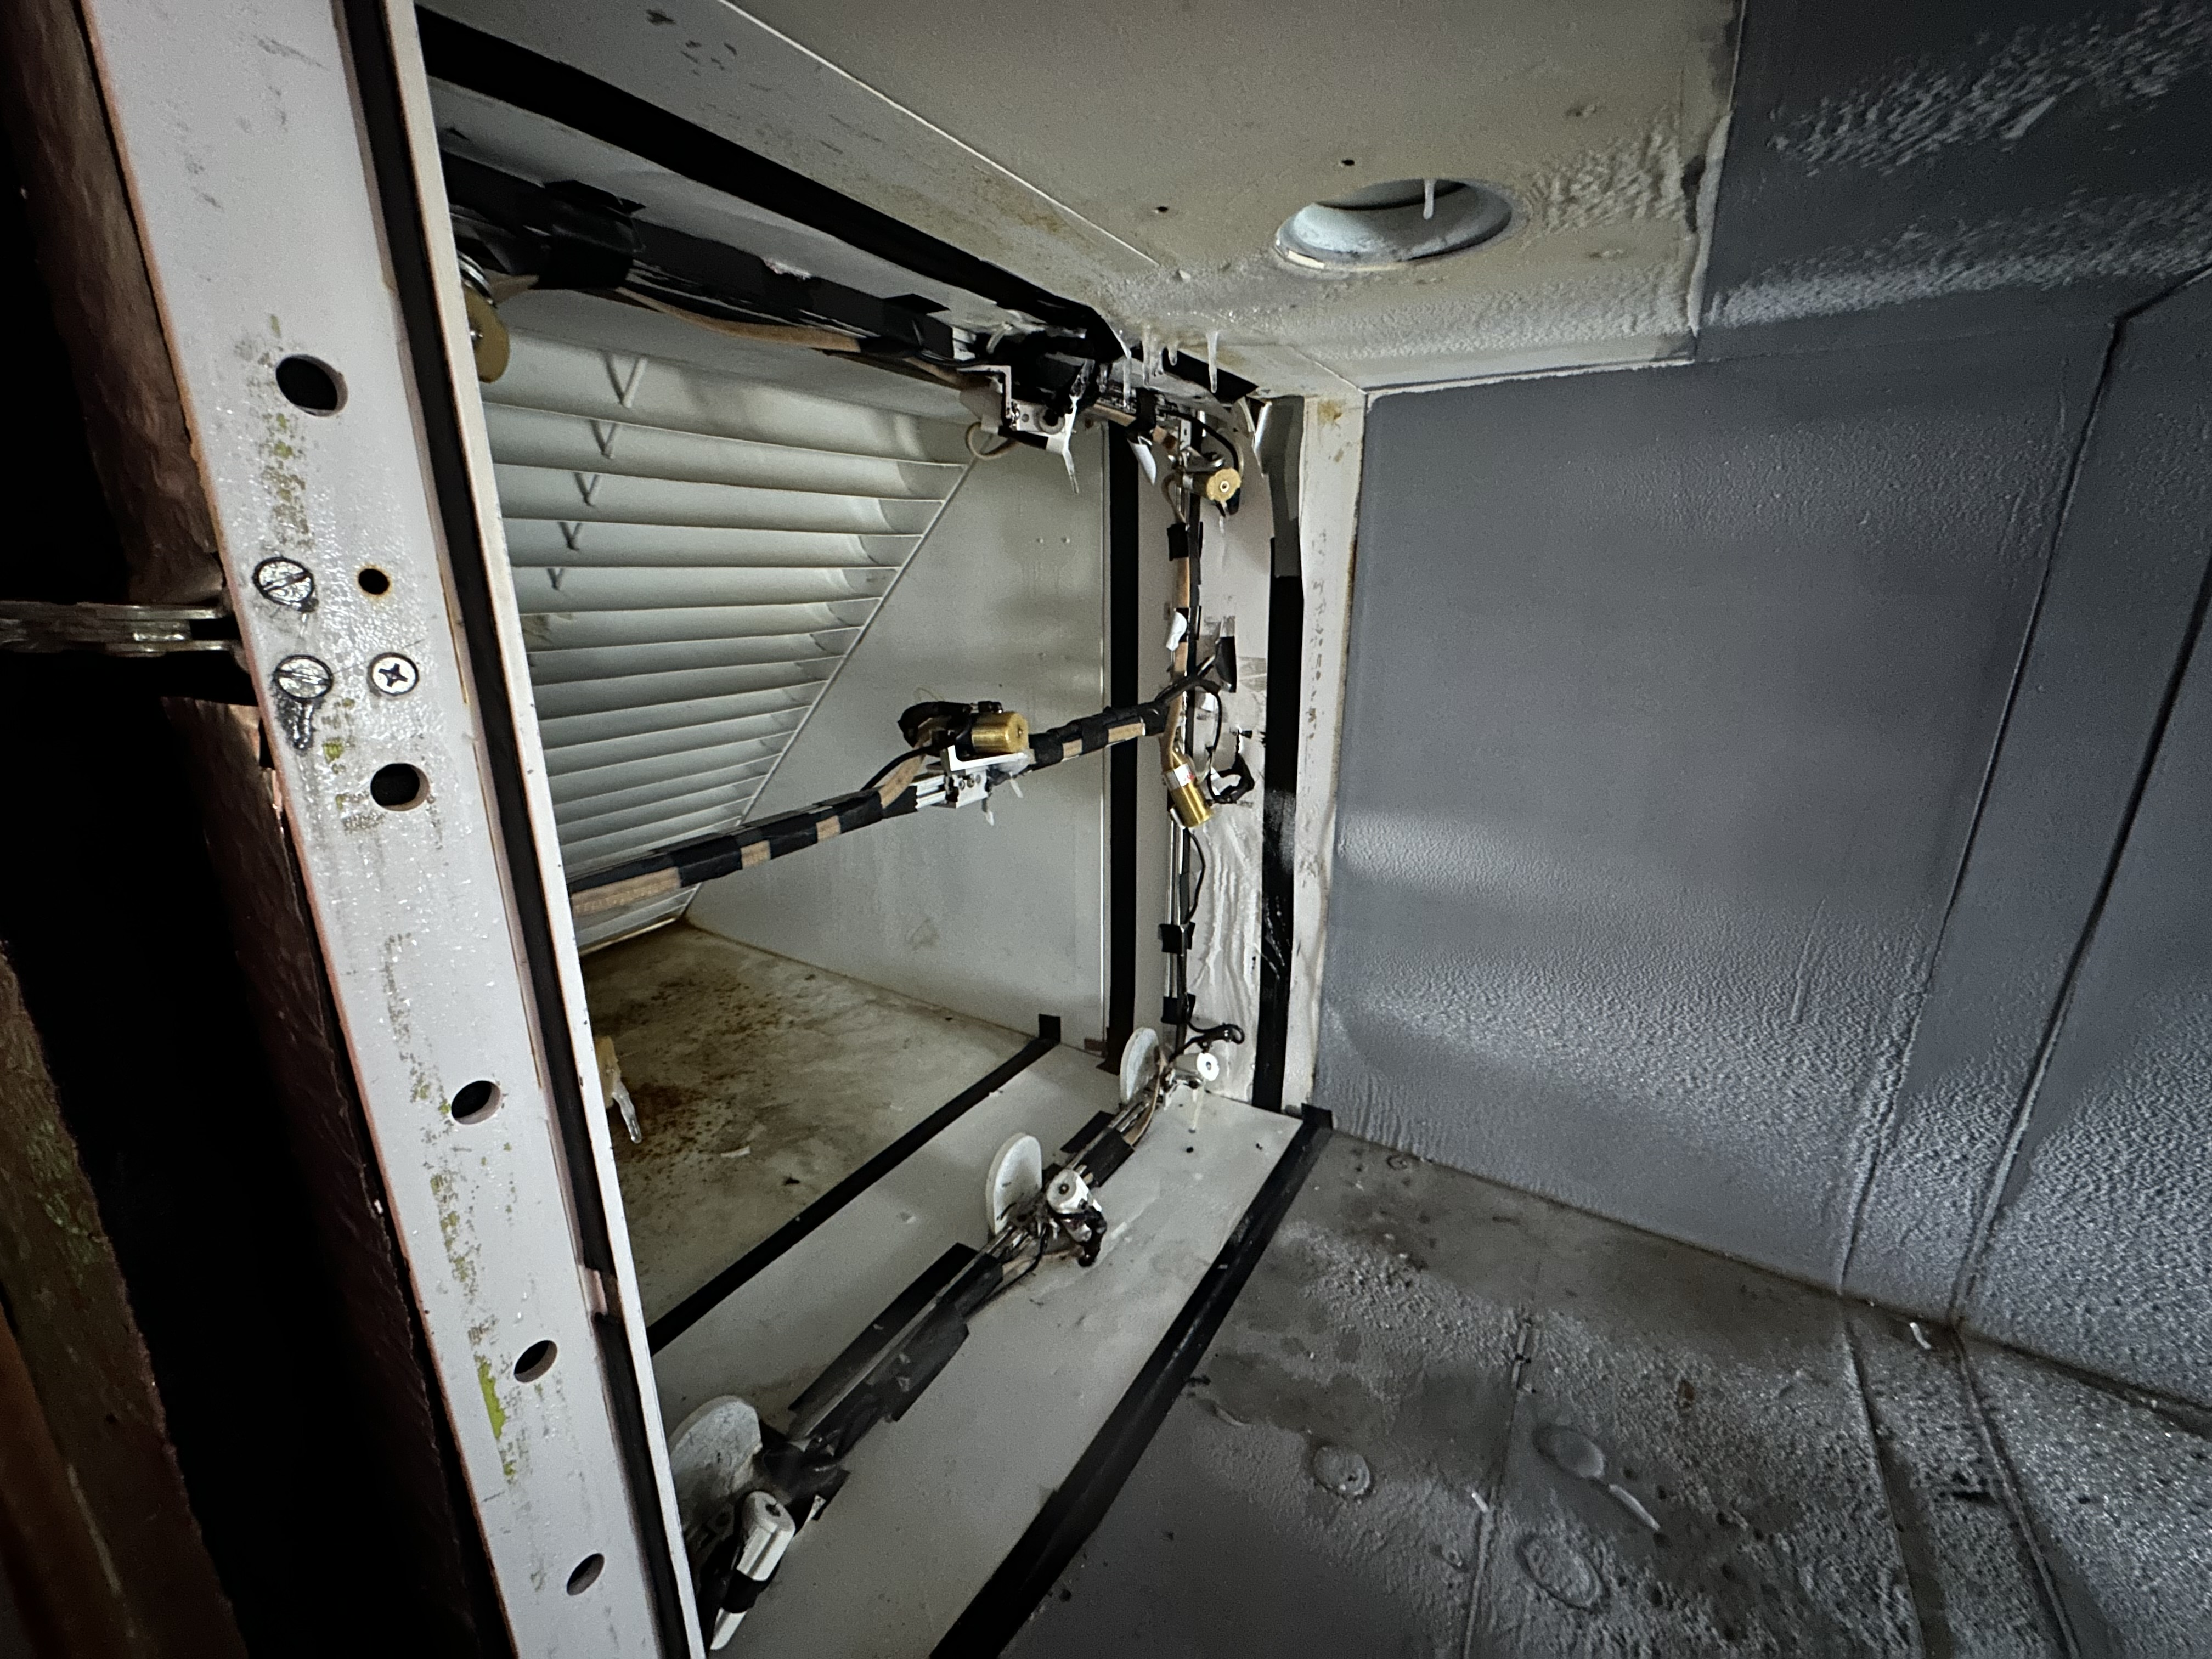
\includegraphics[width=\textwidth]{Figures/IMG_0228.jpeg}
        \caption{Water injection system.}
        \label{fig:water_injector}
    \end{subfigure}    
    \begin{subfigure}{0.49\textwidth}
        \centering
        \includegraphics[width=\textwidth]{Figures/IMG_0229.jpeg}
        \caption{Contraction section.}
        \label{fig:contraction_section}
    \end{subfigure}\\
    \begin{subfigure}{0.49\textwidth}
        \centering
        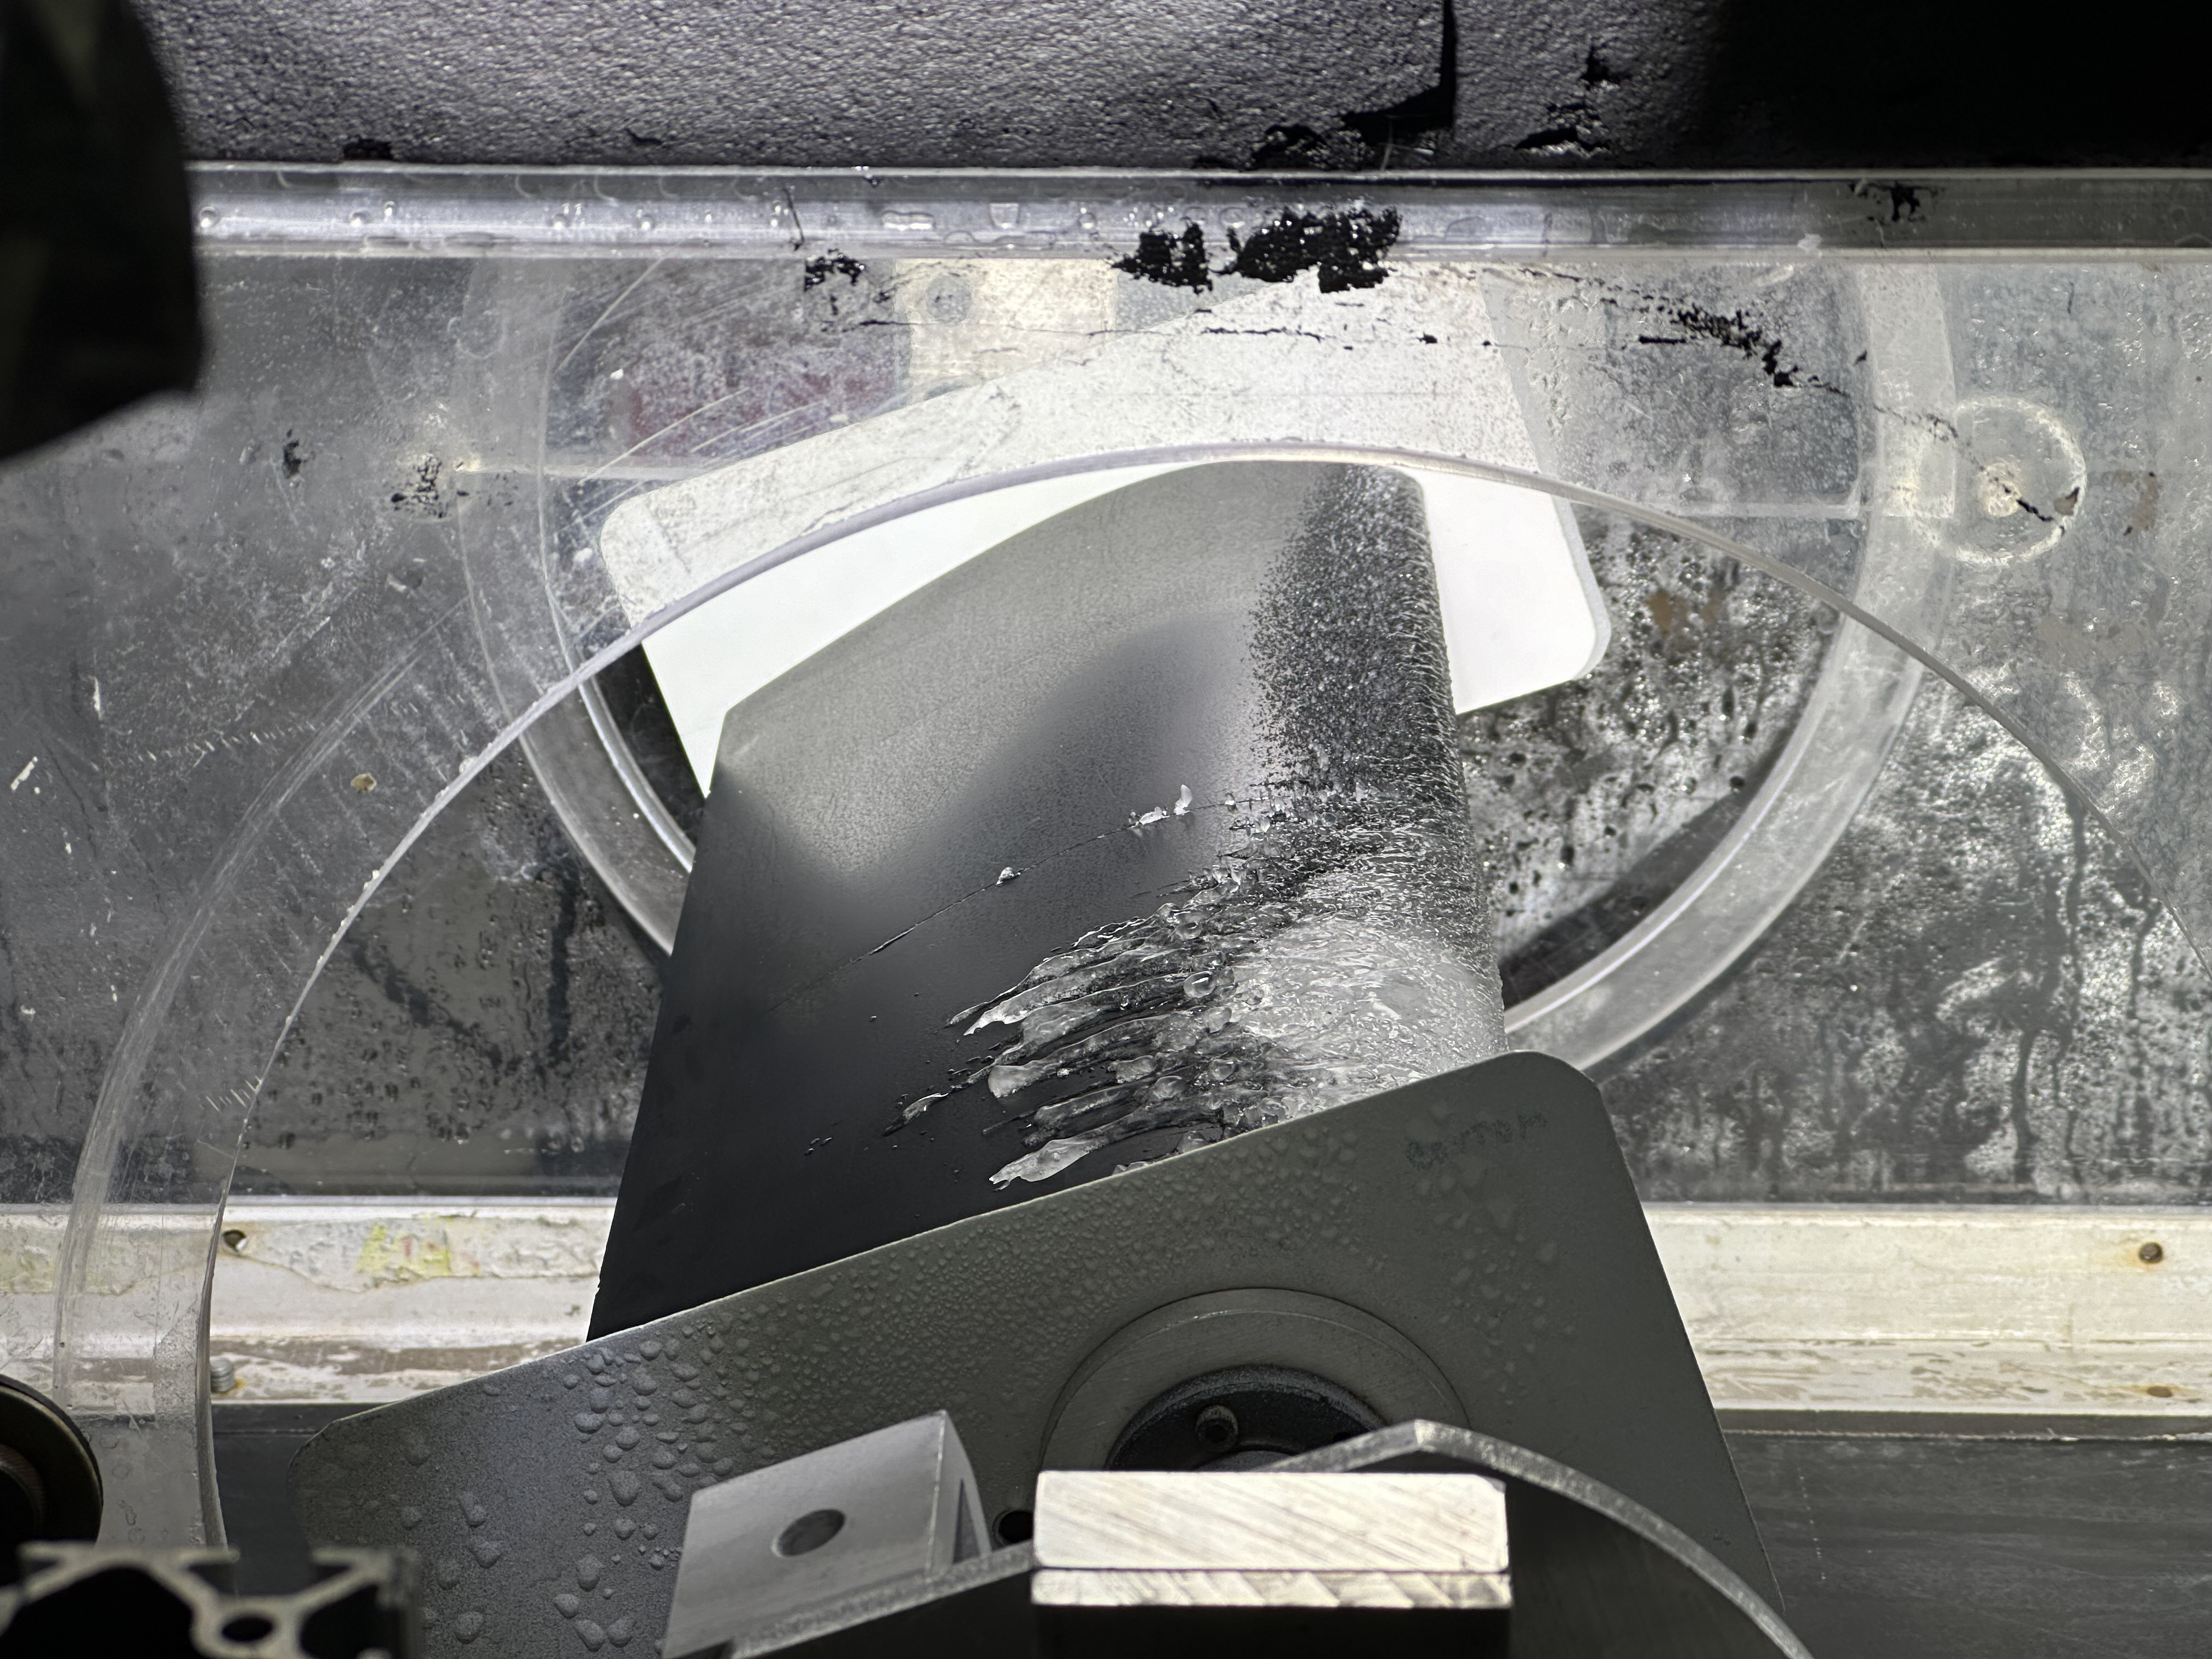
\includegraphics[width=\textwidth]{Figures/IMG_0225.jpeg}
        \caption{Close-up of an iced airfoil.}
        \label{fig:iced_airfoil}
    \end{subfigure}
    \begin{subfigure}{0.49\textwidth}
        \centering
        \includegraphics[width=\textwidth]{Figures/IMG_0217.jpeg}
        \caption{Full icing test apparatus.}
        \label{fig:full_test_apparatus}
    \end{subfigure}
    \caption{Pictures of the icing wind tunnel apparatus.}
    \label{fig:apparatus}
    \vspace*{1.5in}
\end{figure}

\section{Procedures} \label{sec:procedures}

\begin{enumerate}
    \item Turn the wind tunnel on.
    \item Set the \acrshort{aoa} of the airfoil to the first value in the data sheet.
    \item Using the MATLAB application, record data for \qty{10}{\second}. Run this data in the provided processing script to generate values for \gls{c_l}, \gls{c_d}, and \gls{c_m}.
    \item Repeat steps \numrange{2}{3} for all \acrshort{aoa} in the data sheet.
    \item Turn on the water spray system and wait for ice to accrue on the airfoil.
    \item Repeat steps \numrange{2}{3} for all \acrshort{aoa} in the data sheet.
\end{enumerate}

\section{Derivations} \label{sec:derivations}

The data in this lab was collected and processed using a provided \acrfull{matlab} script. This script outputted values for the coefficient of lift, \gls{c_l}, coefficient of drag, \gls{c_d}, and coefficient of moment, \gls{c_m}. This data was plotted using the \acrshort{matlab} script in \autoref{listing:data_analysis_script}. The only calculation required was to calculate the lift to drag ratio, \gls{c_lbyc_d}. This ratio was determined by dividing the \gls{c_l} by the \gls{c_d} for each angle of attack.